\section{Introduction}\label{sec:intro}
% 2026-09-21 house shape (paper-architect, Variant B).  Revised after the cold read of 2026-09-21: the "1" of (1,s) and the
% level k are explained, the example names every level, the limitation is stated in one sentence with a per-vertex figure,
% the peel is described without its technical names, and the query-time claim is one claim (locate in constant time after
% the climb, list at copy speed).  Every number comes from LEDGER.md; the example numbers from tools/example_check.py.

Graphs model relations between entities, and many graph-mining tasks look for groups of vertices that are densely connected inside~\cite{leskovec2016snap,fortunato2010community,Fang2020Survey}.
%
The $k$-core is a standard answer: the largest subgraph in which every vertex has at least $k$ neighbours~\cite{seidman1983network}.
%
% 2026-09-22 cold read (intro): subject and verb together; "the unit" glossed; level k tied to the k of the k-core; "connected through" spelled out; core value named in its own sentence.
The $k$-core counts the neighbours of a vertex.
%
Counting instead the cliques of $s$ vertices that contain the vertex generalizes the $k$-core to a clique size $s$.
%
This is the $(1,s)$-nucleus of Sariy\"uce et al.~\cite{firstNucleus}, where the $1$ says that cliques are counted around single vertices rather than around edges or larger cliques; we call this model the clique core.
%
Choose a clique size $s$ and a level $k$, the $k$ of the $k$-core.
%
The community of a vertex is the largest set containing it in which every vertex lies in at least $k$ cliques of $s$ vertices inside the set.
%
The set is connected through these cliques: any two of its vertices are joined by a sequence of its $s$-cliques in which consecutive cliques share a vertex.
%
Size $2$ gives the connected pieces of the $k$-core, since a clique of two vertices is an edge; size $3$ gives the groups held together by triangles; larger sizes demand denser groups.
%
At a given size, a vertex has a community at every level up to a largest level and at none above it.
%
This largest level is its \emph{core value} at that size.
%
The communities of one size, nested by level, form the \emph{clique-core hierarchy} of that size.
% 2026-09-22 filler pass: "the size is the parameter" was said here, at the end of Example 1.1 and in Applications; kept once, in Applications.

\begin{figure}[t]
\centering
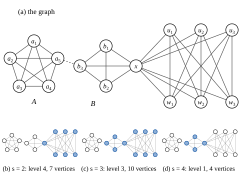
\includegraphics[width=\columnwidth]{figures/fig_running.pdf}
\caption{Running example: (a) the graph, with the $5$-clique $A$, the $4$-clique $B=\{x,b_1,b_2,b_3\}$, six vertices adjacent to $x$, and the edge $a_5b_3$ (dashed), the only edge in no triangle; (b) to (d) the community of $x$ at its core value, for sizes $2$, $3$ and $4$, shaded.}
\label{fig:example}
\end{figure}

\begin{example}\label{ex:intro}
Consider the graph in Figure~\ref{fig:example}.
%
It has a $5$-clique $A=\{a_1,\dots,a_5\}$ and a $4$-clique $B=\{x,b_1,b_2,b_3\}$.
%
It also has a complete bipartite graph between $\{u_1,u_2,u_3\}$ and $\{w_1,w_2,w_3\}$, whose six vertices are all adjacent to $x$.
%
We write $\{u_1,\dots,w_3\}$ for these six.
%
The edge $a_5b_3$ is the only edge between $A$ and the rest of the graph, and it lies in no triangle.
%
% 2026-09-22 filler pass: the example states the three communities and points to the figure; the counts that justify them are Example 2.2.
% 2026-09-22 cold read: A's separateness said once; the 4-clique reason restored; the closing restatement of 7/10/4 removed.
At size $2$, the core value of $x$ is $4$.
%
Its community at level $4$ is $\{x,u_1,\dots,w_3\}$, seven vertices, each with at least four neighbours inside the set, shaded in Figure~\ref{fig:example}(b).
%
At size $3$, the core value of $x$ is $3$.
%
Its community at level $3$ is $B\cup\{u_1,\dots,w_3\}$, ten vertices, each in at least three triangles inside the set, Figure~\ref{fig:example}(c).
%
At size $4$, $x$ lies in one $4$-clique, $B$, since no two of $u_1,u_2,u_3$ and no two of $w_1,w_2,w_3$ are adjacent.
%
Its core value is $1$ and its community at level $1$ is $B$, Figure~\ref{fig:example}(d).
%
The clique $A$ is a community of its own at every size; Example~\ref{ex:nucleus} gives the counts behind these values.
% trace 2026-09-21: tools/example_check.py; neighbours of x: b1,b2,b3,u1..u3,w1..w3 = 9; triangles of x: C(3,2)+3*3 = 12; kappa_2(x)=4, kappa_3(x)=3, kappa_4(x)=1 (make_concept.py 2026-09-22).
\end{example}

\stitle{Applications.}
The size is the parameter a user changes when the groups of one size are too large or too small.
%
\sstitle{Collaboration networks.}
In a coauthorship graph, where vertices are authors and edges join coauthors, the $k$-core around an author covers a broad research area~\cite{newman2001structure,ponomariov2016coauthorship}.
%
The communities at larger sizes keep authors who repeatedly write papers with several of the same people.
%
\sstitle{Co-purchase networks.}
In a product graph, an edge joins two products that are bought together~\cite{linden2003amazon}.
%
The community of a jazz album at its core value is, at size $2$, a $k$-core of more than a hundred thousand products of every kind.
%
At size $3$ it is $23$ albums of the same record label, and at size $5$ the six albums a shop would place on the same shelf (Section~\ref{sec:exp}).
%
\sstitle{Coordinated groups.}
Here the vertices are accounts and an edge joins two accounts that act on the same posts.
%
Accounts that act together on many posts form cliques, and casual interaction rarely forms one~\cite{beutel2013copycatch,hooi2016fraudar}.
%
Larger sizes keep such groups and drop the triangles that arise by chance.

\stitle{Existing methods and their limitations.}
A community query names a vertex $v$, a size $s$ and a level $k$, and asks for the community of $v$ at $(s,k)$.
%
A value query asks only for the core value of $v$ at size $s$.
%
For a fixed size, a community at a higher level lies inside one community at each lower level, and communities at one level are disjoint, so the communities form a tree.
%
% 2026-09-22 cold read: the traversal in two sentences; community search glossed; STrees named as this paper's baseline; "per such size" once.
A depth-first traversal of that tree writes the vertices into an array, each vertex when the traversal reaches the smallest community containing it.
%
Every community is then one contiguous block of the array~\cite{fastHierarchy,Fang2016CLtree}.
%
Existing indexes for community search, the retrieval of the community of a query vertex, store one such tree for one model.
%
The model is the $k$-core~\cite{Barbieri2015ShellStruct,Fang2016CLtree}, the $k$-truss, the same idea with edges in place of vertices~\cite{huang2014truss,akbas2017truss}, or the clique cores of one clique size~\cite{fastHierarchy}.
%
An index for every size then holds \textbf{\textit{one hierarchy per size}}.
%
We call this index \strees and use it as the baseline of the experiments.
%
Call the size of the largest clique containing a vertex its clique number.
%
A vertex lies in cliques of every size from $2$ to its clique number, so \strees stores it in the array of every such size and keeps a core value for each.
%
On the web graph \webuk, cliques reach $500$ vertices and a vertex lies in $181$ arrays on average.
%
The index \strees takes $190$~MB for $129{,}632$ vertices, or $1.5$~KB per vertex.
%
On the coauthorship graph \textsf{ca-coauthors-dblp}, with cliques of $337$ vertices, it takes $202$~MB for $540{,}486$ vertices.
%
The alternative is to keep no index and to decompose the graph at the queried size when the query arrives, which costs seconds to minutes per query on these graphs.
%
The counting-based decomposition \cnd~\cite{Zhang2026NucleusCounting} needs $15.7$ hours to cover the $499$ sizes of \webuk once.

\stitle{Research question.}
This leads to the question this paper answers: \textbf{\textit{how to index the clique-core hierarchies of every size at once, storing each vertex once and returning every community as a few ranges of consecutive ids?}}

\stitle{Challenges.}
For one size, the tree of that size meets both demands.
%
Across sizes, the question raises three difficulties.
%
\sstitle{Repetition across sizes.}
Within one size, two vertices that lie in the same community at every level are interchangeable and could share one record.
%
However, the communities of a vertex change from size to size.
%
Two vertices that share every community at size $2$ may lie in different communities at size $3$.
%
The first difficulty is to decide which vertices can share one record for every size, every level and every query without losing an answer.
%
\sstitle{Contiguity of communities.}
Once vertices are grouped, a community is a set of groups rather than one block of an array.
%
However, the depth-first order of one size lists the groups in one order and that of another size in another.
%
A community, a set of groups, then does not come out as a few ranges of ids.
%
The second difficulty is to return any community of any size as a few ranges of ids, in constant time per range.
%
\sstitle{Construction of every size.}
The tree of one size is the output of one decomposition of the graph.
%
However, the sizes are many, cliques reach hundreds of vertices, and the decompositions of all sizes together cost hours.
%
The third difficulty is to build the trees of all sizes from one computation.

\stitle{Our idea.}
We start from the queries and ask which pairs of vertices no query can tell apart.
%
\sstitle{Chains.}
Two vertices are \emph{hierarchy-equivalent} when they have the same core value at every size and lie in the same community at every size and level.
%
The \emph{own node} of a vertex at a size is its community at its core value, the deepest node of the tree of that size that contains the vertex.
%
We prove that two vertices are hierarchy-equivalent exactly when they have the same own node at every size (Theorem~\ref{thm:chains}).
%
We call the classes of hierarchy-equivalent vertices \emph{chains}, since a class follows one chain of own nodes through the sizes.
%
Every community is a union of chains, and no partition into larger groups answers every query (Proposition~\ref{prop:coarsest}).
%
On \dblp, $13{,}459$ chains hold its $317{,}080$ vertices, so one record serves $24$ vertices on average.
%
% 2026-09-22 filler pass: each idea says what it does and what it buys; the mechanics (entries, runs as maximal stretches, the climb, the binomial bound) are Section 5.
\sstitle{Aligned labels, chain order and run arrays.}
% 2026-09-22 cold read: labels = new ids; the ranking rule spelled out; runs in their own sentence; the climb named with its cost; "through the vertex" in the floor; values under their own sstitle.
We give the vertices new ids, their \emph{labels}, so that every chain is one interval of labels.
%
We rank the chains by the depth-first positions of their own nodes, comparing the positions at size $2$ first and breaking ties at size $3$, $4$ and so on.
%
Every size-$2$ community is then one range of labels (Theorem~\ref{thm:onerange}), and at larger sizes the same order keeps the number of ranges small (Table~\ref{tab:queries}).
%
For each size, the index stores the tree of that size, with the chains in place of the vertices, and the order in which a depth-first traversal of the tree lists the chains.
%
Consecutive labels in this order are merged into \emph{runs}.
%
A community query climbs the tree of its size from the own node of the vertex to the node of the queried level, $O(\log d)$ steps for $d$ levels (Section~\ref{sec:queries}).
%
That node's community is a first range, whole runs and a last range, located in constant time and reported in constant time per range (Theorem~\ref{thm:retrieval}).
%
\sstitle{Values.}
At every size $s$, the core value of a vertex is at least the number of $s$-cliques through it inside a largest clique containing it, a binomial coefficient of its clique number.
%
Once the value equals this number at one size, it does so at every larger size (Theorem~\ref{thm:tail}), and the index stores values only below that size.
%
\sstitle{One clique tree for every size.}
A clique tree~\cite{Pivoter}, a compact representation of all cliques of a graph, gives for every vertex and every size the number of cliques of that size through the vertex.
%
The values of one size come from a peel.
%
Vertices are removed one at a time in increasing order of their clique counts, and the largest count seen so far at a removal is the core value of the removed vertex.
%
Each size first replays the removal order of the previous size, and a check on clique counts tells whether the result is exact (Theorem~\ref{thm:replay}).
%
Otherwise the size is peeled from scratch, and its own removal order is tried at the next size.

\stitle{Contributions.}
% 2026-09-22 filler pass + cold read: one sentence per deliverable with its theorems, no mechanics (they are "Our idea"); graphs named; "locates" glossed; ns spelled out.
\sstitle{Chains.}
Theorem~\ref{thm:chains} decides hierarchy equivalence from the own nodes alone, and Proposition~\ref{prop:coarsest} shows that the chains are the coarsest partition that loses no answer.
%
\sstitle{The chain index.}
\chainidx stores each vertex once and returns every community as label ranges: one range at size $2$ (Theorem~\ref{thm:onerange}), and at every size a list located in constant time after the climb (Theorem~\ref{thm:retrieval}).
%
Core values are stored only below the size from which they equal a binomial coefficient (Theorem~\ref{thm:tail}).
%
\sstitle{Construction from one clique tree.}
Our algorithm \build computes the index of every size from one clique tree, replaying the removal order of one size at the next when a check on clique counts proves the replay exact (Theorem~\ref{thm:replay}).
%
Its working memory is the clique tree plus space linear in the vertices and the chains.
%
\sstitle{Experimental evaluation.}
\chainidx is \ratiomin$\times$ to \ratiomax$\times$ smaller than \strees on \numgraphs{} graphs from five families (median \ratiomedian$\times$).
%
It locates a community, that is, finds its ranges, in \locmin{} to \locmax{} nanoseconds.
%
Listing the vertices takes \stmininv{} to \stmaxinv{} times the time of a memory copy of the answer (median \stmedianinv).
%
It is built for every size \priormin$\times$ to \priormax$\times$ faster than one decomposition per size (median \priormedian$\times$).
%
Two case studies on graphs whose vertices carry names and categories show the effect of the size.
%
On \dblp the size that best matches a community given with the graph as ground truth changes from query to query.
%
On the product graph \textsf{com-amazon} the size narrows a community from a store to a shelf.

\stitle{Organization.}
% 2026-09-22 filler pass: two sentences.
Section~\ref{sec:prelim} gives the definitions and Section~\ref{sec:strees} the cost of one hierarchy per size.
%
Sections~\ref{sec:chains} to~\ref{sec:construction} give the chains, the index, its queries and its construction, Section~\ref{sec:exp} the experiments and Section~\ref{sec:related} related work.
